\documentclass[12pt]{article}
\usepackage{amsmath}
\usepackage{graphicx}
\usepackage{hyperref}
\usepackage{listings}
\usepackage{color}
\usepackage{pythonhighlight}

\title{Operating System Course Report - First Half of the Semester}
\author{B class}
\date{\today}

\begin{document}

\maketitle
\newpage

\tableofcontents
\newpage

\section{Introduction}
This report summarizes the topics covered during the first half of the Operating System course. It includes theoretical concepts, practical implementations, and assignments. The course focuses on the fundamentals of operating systems, including system architecture, process management, CPU scheduling, and deadlock handling.

\section{Course Overview}
\subsection{Objectives}
The main objectives of this course are:
\begin{itemize}
    \item To understand the basic components and architecture of a computer system.
    \item To learn process management, scheduling, and inter-process communication.
    \item To explore file systems, input/output management, and virtualization.
    \item To study the prevention and handling of deadlocks in operating systems.
\end{itemize}

\subsection{Course Structure}
The course is divided into two halves. This report focuses on the first half, which covers:
\begin{itemize}
    \item Basic Concepts and Components of Computer Systems
    \item System Performance and Metrics
    \item System Architecture of Computer Systems
    \item Process Description and Control
    \item Scheduling Algorithms
    \item Process Creation and Termination
    \item Introduction to Threads
    \item File Systems
    \item Input and Output Management
    \item Deadlock Introduction and Prevention
    \item User Interface Management
    \item Virtualization in Operating Systems
\end{itemize}

\section{Topics Covered}

\subsection{Basic Concepts and Components of Computer Systems}
This section explains the fundamental components that make up a computer system, including the CPU, memory, storage, and input/output devices.

\subsection{System Performance and Metrics}
This section introduces various system performance metrics used to measure the efficiency of a computer system, including throughput, response time, and utilization.

\subsection{System Architecture of Computer Systems}
Describes the architecture of modern computer systems, focusing on the interaction between hardware and the operating system.

\subsection{Process Description and Control}
Processes are a central concept in operating systems. This section covers:
\begin{itemize}
    \item Process states and state transitions
    \item Process control block (PCB)
    \item Context switching
\end{itemize}

\subsection{Scheduling Algorithms}
This section covers:
\begin{itemize}
    \item First-Come, First-Served (FCFS)
    \item Shortest Job Next (SJN)
    \item Round Robin (RR)
\end{itemize}
It explains how these algorithms are used to allocate CPU time to processes.

\subsection{Process Creation and Termination}
Details how processes are created and terminated by the operating system, including:
\begin{itemize}
    \item \textit{Process spawning}
    \item \textit{Process termination conditions}
    \subsubsection{Sumber Daya Proses}

    \paragraph{A. Alokasi Memori} \mbox{} \\
    Setiap proses memerlukan memori untuk menyimpan data dan instruksi yang akan dijalankannya. Sistem operasi bertanggung jawab untuk mengalokasikan memori ini kepada proses dan memastikan bahwa proses lain tidak mengakses memori yang dialokasikan secara ilegal.

    \begin{itemize}
        \item Jenis memori yang dialokasikan:
        \begin{enumerate}
            \item \textit{Stack:} Digunakan untuk menyimpan variabel lokal dan melacak fungsi yang dipanggil selama eksekusi program.
            \item \textit{Heap:} Menyediakan memori dinamis untuk aplikasi, digunakan saat proses memerlukan memori yang dialokasikan secara dinamis selama \textit{runtime}.
            \item \textit{Segmen Kode (Text Segment):} Menyimpan instruksi yang akan dieksekusi oleh CPU. Ini adalah bagian dari memori yang bersifat read-only, sehingga   mencegah modifikasi terhadap instruksi program.
        \end{enumerate}
    \end{itemize}

    \paragraph{B. Penjadwalan Waktu CPU} \mbox{} \\
    Sistem operasi mengatur bagaimana dan kapan setiap proses dapat menggunakan CPU. Karena jumlah CPU terbatas dan banyak proses yang berjalan secara bersamaan, sistem operasi menggunakan mekanisme penjadwalan untuk mengalokasikan waktu CPU secara adil dan efisien.

    \begin{itemize}
        \item Jenis Penjadwalan Waktu CPU:
        \begin{enumerate}
            \item \textit{Preemptive Scheduling:} Sistem operasi dapat menghentikan proses yang sedang berjalan dan memberikan CPU kepada proses lain yang lebih prioritas.
            \item \textit{Non-Preemptive Scheduling:} Proses diberikan CPU sampai selesai atau secara sukarela melepaskan CPU, baru setelah itu sistem operasi memberikan CPU ke proses lain.
        \end{enumerate}
    \end{itemize}

    \paragraph{C. Pengaturan \textit{File Descriptors}} \mbox{} \\
    \textit{File descriptor} adalah integer unik yang diberikan oleh sistem operasi untuk merujuk ke \textit{file}, \textit{socket}, atau perangkat yang dibuka oleh proses. Proses menggunakan \textit{file descriptor} untuk melakukan operasi I/O seperti membaca, menulis, atau mengelola \textit{file}.

    \begin{itemize}
        \item Fungsi \textit{File Descriptor}:
        \begin{enumerate}
            \item {Akses File:}  \textit{File descriptors} digunakan oleh proses untuk membaca, menulis, atau melakukan operasi lainnya pada \textit{file}.
            \item Komunikasi Antar-Proses (IPC): \textit{File descriptors} digunakan dalam komunikasi antar-proses seperti socket atau pipe untuk mengirimkan data antar proses.
            \item Manajemen Sumber Daya: \textit{File descriptors} membantu sistem operasi melacak dan mengelola sumber daya seperti \textit{file} terbuka, socket, atau perangkat yang digunakan oleh suatu proses.
        \end{enumerate}
    \end{itemize}

    \subsubsection{Terminasi Paksa oleh Proses Lain}

    \paragraph{A. \textit{Sinyal Kill}} \mbox{} \\
    \textit{Sinyal Kill} adalah perintah yang digunakan dalam sistem operasi untuk menghentikan proses yang sedang berjalan. Meskipun namanya terdengar drastis, sinyal ini tidak selalu berarti menghentikan proses secara paksa, ada berbagai jenis sinyal yang dapat dikirim.

    Contoh Sinyal:
    \begin{enumerate}
        \item \textit{SIGTERM:} Sinyal ini memberi tahu proses untuk berhenti dengan cara yang teratur. Proses dapat menangani sinyal ini dengan melakukan pembersihan sebelum keluar.
        \item \textit{SIGKILL:} Sinyal ini menghentikan proses secara paksa dan tidak dapat diabaikan atau ditangani oleh proses. Ini digunakan ketika proses tidak merespons permintaan untuk berhenti.
    \end{enumerate}

    Penggunaan \textit{Sinyal Kill}:  
    \newline Sinyal ini biasanya digunakan ketika proses tidak merespons, macet, atau berperilaku tidak sesuai. Misalnya, jika aplikasi grafis tidak merespons, pengguna dapat menggunakan perintah \textit{kill} untuk menghentikannya.

    \paragraph{B. \textit{Timeout}} \mbox{} \\
    \textit{Timeout} adalah mekanisme di mana sistem operasi menetapkan batas waktu tertentu untuk proses. Jika proses tidak menyelesaikan tugasnya dalam jangka waktu yang ditentukan, sistem operasi akan menghentikannya.

    Contoh Penggunaan:  
    Dalam sistem waktu nyata atau dalam lingkungan penjadwalan pekerjaan, jika sebuah proses tidak merespons dalam waktu tertentu, sistem operasi dapat mengakhiri proses tersebut untuk mencegah masalah dalam pengelolaan sumber daya.

    Pentingnya \textit{Timeout:}  \\
    \textit{Timeout} mencegah satu proses dari penggunaan sumber daya sistem yang berlebihan, yang bisa mengakibatkan penurunan kinerja untuk proses lain.

    \subsubsection{\textit{Orphan Process} atau \textit{Zombie Process}}

    \begin{figure}[h]
	\centering
	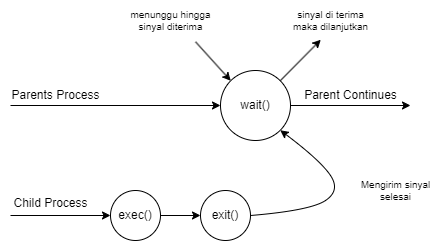
\includegraphics[width=1\textwidth]{asset/Process.png}
	\label{fig:gambar}
    \end{figure}

    \paragraph{A. \textit{Orphan Process}} \mbox{} \\
    \textit{Orphan Process} adalah proses anak yang tetap berjalan setelah proses induknya berakhir. Ketika proses induk mati, proses anak menjadi yatim, tetapi sistem operasi tidak langsung menghapusnya.

    Pengelolaan \textit{Orphan Process}:  
    Dalam sistem berbasis Unix, \textit{Orphan Process} diadopsi oleh proses init (PID 1). Proses init bertugas untuk mengelola \textit{orphan process} dan memastikan bahwa semua sumber daya yang dialokasikan untuk proses anak dibebaskan saat proses tersebut berakhir.

    \paragraph{B. \textit{Zombie Process}} \mbox{} \\
    \textit{Zombie Process} adalah proses yang telah selesai eksekusi tetapi masih ada dalam tabel proses karena proses induknya belum mengambil status keluar (exit status)nya. Proses ini tidak aktif, tetapi masih ada dalam sistem. 

    Proses zombie muncul karena sistem operasi menyimpan informasi tentang proses yang telah selesai sehingga proses induk dapat mendapatkan status keluar untuk melakukan pembersihan yang diperlukan.

    Menghapus Proses Zombie:
    Setelah proses induk menggunakan \texttt{wait()} atau \texttt{waitpid()} untuk mengambil status keluar dari proses anaknya, sistem operasi dapat menghapus entri proses zombie dari tabel proses.

    \subsubsection{Tahapan dalam Terminasi Proses}

    \paragraph{A. Sinyal untuk Terminasi}\mbox{}\\
    Proses dapat berakhir dengan cara alami atau menerima sinyal untuk terminasi. Jika menerima sinyal, proses akan melaksanakan handler (jika ada) atau menghentikan eksekusinya.
        
    \paragraph{B. Pembersihan Sumber Daya} \mbox{} \\
    Setelah proses menerima sinyal terminasi atau selesai eksekusi, sistem operasi akan mulai mereklamasi semua sumber daya yang digunakan oleh proses tersebut. Ini termasuk:
    \begin{enumerate}
        \item \textit{Memori:} Menghapus alokasi memori yang digunakan oleh stack, heap, dan segmen kode.
        \item \textit{File Deskriptor:} Menutup semua file yang dibuka oleh proses untuk mencegah kebocoran sumber daya.
        \item Perangkat I/O: Mengembalikan kontrol atas perangkat I/O yang digunakan oleh proses.
    \end{enumerate}
        
    \paragraph{C. Penghapusan \textit{Process Control Block} (PCB)}  
    \mbox{}\\ Setiap proses memiliki PCB yang menyimpan informasi penting tentang proses, termasuk status, prioritas, dan informasi penggunaan sumber daya. Setelah proses dibersihkan, PCB dihapus dari tabel proses untuk membebaskan ruang dan menghilangkan informasi tentang proses tersebut.
        
    \paragraph{D. Pemberitahuan kepada Proses Induk}\mbox{} \\ 
    Dalam sistem berbasis Unix, setelah proses anak selesai, proses induknya diberi tahu melalui sinyal \texttt{SIGCHLD}. Proses induk dapat menangani sinyal ini dan memanggil \texttt{wait()} atau \texttt{waitpid()} untuk mengambil status keluar dari proses anak. Ini memungkinkan proses induk untuk melakukan pembersihan yang diperlukan dan memastikan bahwa tidak ada proses zombie yang tertinggal.

    \textbf{Daftar Pustaka}
    \begin{itemize}
        \item Silberschatz, A., Galvin, P. B., & Gagne, G. (2018). Operating system concepts (10th ed.). Wiley.
        \item Almaunah. (n.d.). Mengidentifikasi Proses Sistem Operasi. Fakultas Komputer, Universitas Mitra Indonesia.
    \end{itemize}
\end{itemize}

\subsection{Introduction to Threads}
This section introduces the concept of threads and their relation to processes, covering:
\begin{itemize}
    \item Single-threaded vs. multi-threaded processes
    \item Benefits of multithreading
\end{itemize}

\begin{figure}[h]
    \centering
    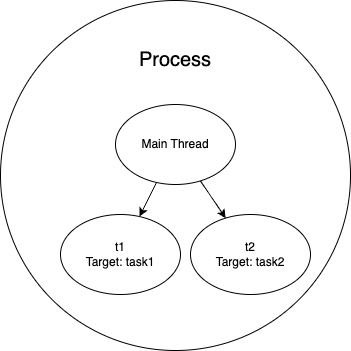
\includegraphics[width=0.5\textwidth]{/Users/khawaritzmi/Unhas/os_report_mid2024/b_class/asset/example.png}  % Sesuaikan nama file dan ukurannya
    \caption{Ini adalah gambar contoh dari multithreading.}
    \label{fig:contoh_gambar}
\end{figure}

Seperti yang terlihat pada Gambar \ref{fig:contoh_gambar}, inilah cara menambahkan gambar dengan keterangan.

\subsection{File Systems}
File systems provide a way for the operating system to store, retrieve, and manage data. This section explains:
\begin{itemize}
    \item File system structure
    \item File access methods
    \item Directory management
\end{itemize}

\subsection{Input and Output Management}
Input and output management is key for handling the interaction between the system and external devices. This section includes:
\begin{itemize}
    \item Device drivers
    \item I/O scheduling
\end{itemize}

\subsection{Deadlock Introduction and Prevention}
Explores the concept of deadlocks and methods for preventing them:
\begin{itemize}
    \item Deadlock conditions
    \item Deadlock prevention techniques
\end{itemize}

\subsection{User Interface Management}
This section discusses the role of the operating system in managing the user interface. Topics covered include:
\begin{itemize}
    \item Graphical User Interface (GUI)
    \item Command-Line Interface (CLI)
    \item Interaction between the user and the operating system
\end{itemize}

\subsection{Virtualization in Operating Systems}
Virtualization allows multiple operating systems to run concurrently on a single physical machine. This section explores:
\begin{itemize}
    \item Concept of virtualization
    \item Hypervisors and their types
    \item Benefits of virtualization in modern computing
\end{itemize}

\section{Assignments and Practical Work}
\subsection{Assignment 1: Process Scheduling}
Students were tasked with implementing various process scheduling algorithms (e.g., FCFS, SJN, and RR) and comparing their performance under different conditions.
\subsubsection{Group 1}
\begin{python}
    class Process:
    def __init__(self, pid, arrival_time, burst_time):
        self.pid = pid
        self.arrival_time = arrival_time
        self.burst_time = burst_time
        self.completion_time = 0
        self.turnaround_time = 0
        self.waiting_time = 0
\end{python}

\begin{table}[htbp] % Optional: For floating position
    \centering
    \begin{tabular}{|c|c|c|} % Defines number of columns and alignment (c = center, l = left, r = right). '|' creates vertical lines.
    \hline
    Header 1 & Header 2 & Header 3 \\ % Column headers
    \hline
    Row 1, Column 1 & Row 1, Column 2 & Row 1, Column 3 \\ % First row of data
    \hline
    Row 2, Column 1 & Row 2, Column 2 & Row 2, Column 3 \\ % Second row of data
    \hline
    \end{tabular}
    \caption{Your table caption} % Optional: For adding a caption
    \label{tab:your_label} % Optional: For cross-referencing the table
\end{table}

\subsection{Assignment 2: Deadlock Handling}
In this assignment, students were asked to simulate different deadlock scenarios and explore various prevention methods.

\subsection{Assignment 3: Multithreading and Amdahl's Law}
This assignment involved designing a multithreading scenario to solve a computationally intensive problem. Students then applied **Amdahl's Law** to calculate the theoretical speedup of the program as the number of threads increased.

\subsubsection{group 1}
\subsubsection{group 2}
\subsubsection{group 3}
\subsubsection{group 4}
\subsubsection{group 5}
\subsubsection{group 6}
Buatlah sebuah program Python untuk menghitung nilai Fibonacci ke-40 menggunakan multithreading. Setelah itu, implementasikan Amdahl's Law untuk menghitung speedup teoretis dengan berbagai jumlah thread.
Jawaban:

\begin{python}
import threading
import time

# Fungsi untuk menghitung Fibonacci secara rekursif
def hitung_fibonacci(angka):
    if angka <= 1:
        return angka
    else:
        return hitung_fibonacci(angka-1) + hitung_fibonacci(angka-2)

# Fungsi untuk mengukur waktu eksekusi
def jalankan_threads(jumlah_threads, angka_fibonacci):
    threads = []
    
    waktu_mulai = time.time()
    
    for i in range(jumlah_threads):
        thread = threading.Thread(target=hitung_fibonacci, args=(angka_fibonacci,))
        threads.append(thread)
        thread.start()

    for thread in threads:
        thread.join()
    
    waktu_selesai = time.time()
    return waktu_selesai - waktu_mulai

# Implementasi Amdahl's Law
def hitung_speedup_amdahl(persentase_paralel, jumlah_threads):
    return 1 / ((1 - persentase_paralel) + (persentase_paralel / jumlah_threads))

# Main program
if __name__ == "__main__":
    angka_fibonacci = 40  # Fibonacci ke-40
    persentase_paralel = 0.95  # Estimasi paralelisme
    daftar_threads = [1, 2, 4, 8]  # Daftar jumlah thread yang akan diuji
    
    for jumlah_threads in daftar_threads:
        waktu_eksekusi = jalankan_threads(jumlah_threads, angka_fibonacci)
        speedup_teoretis = hitung_speedup_amdahl(persentase_paralel, jumlah_threads)
        
        print(f"\nJumlah Threads: {jumlah_threads}")
        print(f"Waktu Eksekusi: {waktu_eksekusi:.4f} detik")
        print(f"Speedup Teoretis (Amdahl's Law): {speedup_teoretis:.4f}")
\end{python}

\subsection{Assignment 4: Simple Command-Line Interface (CLI) for User Interface Management}
Students were tasked with creating a simple **CLI** for user interface management. The CLI should support basic commands such as file manipulation (creating, listing, and deleting files), process management, and system status reporting.

\subsection{Assignment 5: File System Access}
In this assignment, students implemented file system access routines, including:
\begin{itemize}
    \item File creation and deletion
    \item Reading from and writing to files
    \item Navigating directories and managing file permissions
\end{itemize}

\section{Conclusion}
The first half of the course introduced core operating system concepts, including process management, scheduling, multithreading, and file system access. These topics provided a foundation for more advanced topics to be covered in the second half of the course.

\end{document}